\subsection{Ordenamiento de Arreglos}

Para analizar los algoritmos de ordenamiento, nos vamos a enfocar en las gráficas del dominio D7, ya que muestran las mismas tendencias que el D1 pero dejan ver mejor cómo afecta la distribución inicial de los datos al rendimiento.

Revisando el \textbf{tiempo de ejecución} (Figura \ref{fig:sort_tiempo}) con escala Log10, se nota claramente que \texttt{ Merge Sort} (línea azul) es sumamente estable. Se mantiene en su cota $\mathcal{O}(n \log n)$ sin importar si el arreglo viene ordenado, aleatorio o invertido. En cambio, \texttt{Quick Sort} (línea roja) rinde muy bien con datos aleatorios, pero rinde pésimo y cae en su peor caso $\mathcal{O}(n^2)$ cuando el arreglo ya viene ordenado o invertido. Por este motivo, se optó por no correr las pruebas de $N=10^7$ para esos casos, ya que iban a tardar más de 4 horas. Por último, \texttt{sort} (línea verde) soluciona esto gracias a que implementa \textit{Introsort}, logrando los mismos tiempos de Quick Sort pero sin caerse en los peores escenarios.

\begin{figure}[H]
    \centering
    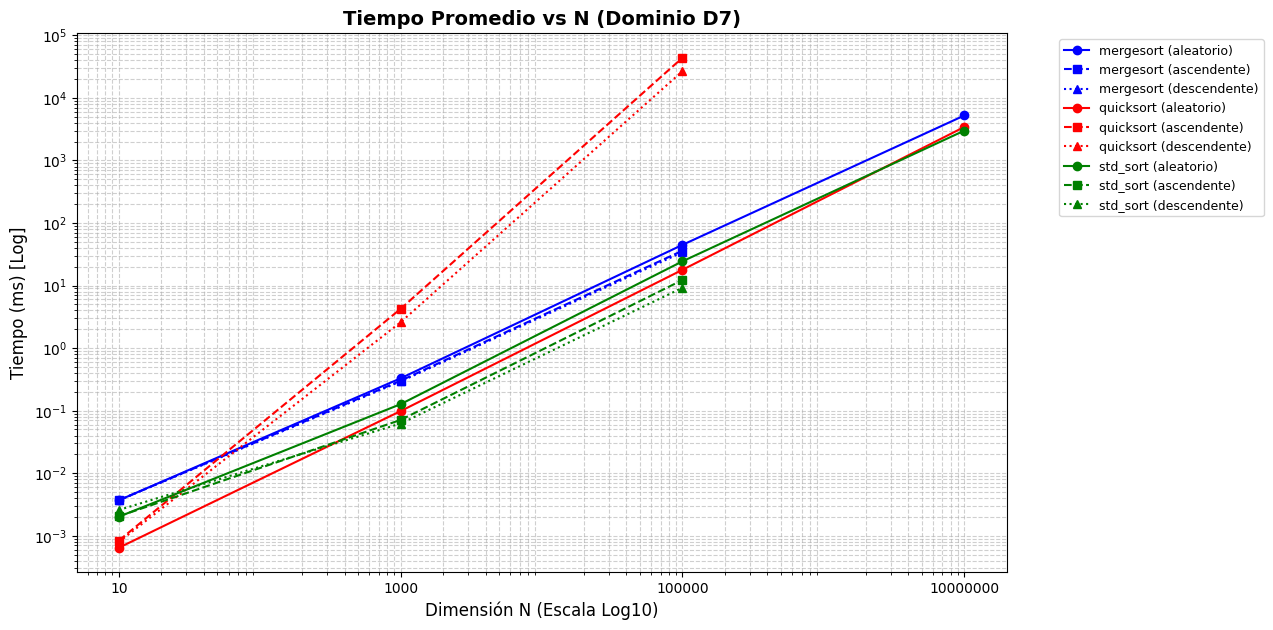
\includegraphics[width=0.75\textwidth]{../code/sorting/plots/tiempo_vs_n_D7.png}
    \caption{Tiempos promedio de ejecución en ordenamiento (Dominio D7). Se nota el salto cuadrático de Quick Sort con datos ordenados.}
    \label{fig:sort_tiempo}
\end{figure}

Respecto a la \textbf{memoria consumida} (Figura \ref{fig:sort_mem}), la escala \texttt{SymLog} permite ver claramente que \texttt{Quick Sort} y \texttt{sort} operan de forma similar. Sus curvas son iguales porque solo usan la memoria del arreglo original más el pequeño costo de la pila de recursión ($\mathcal{O}(\log n)$). Por otro lado, \texttt{Merge Sort} necesita crear arreglos auxiliares para mezclar los datos, sumando un costo extra de $\mathcal{O}(n)$ que dispara su consumo frente al resto.

\begin{figure}[H]
    \centering
    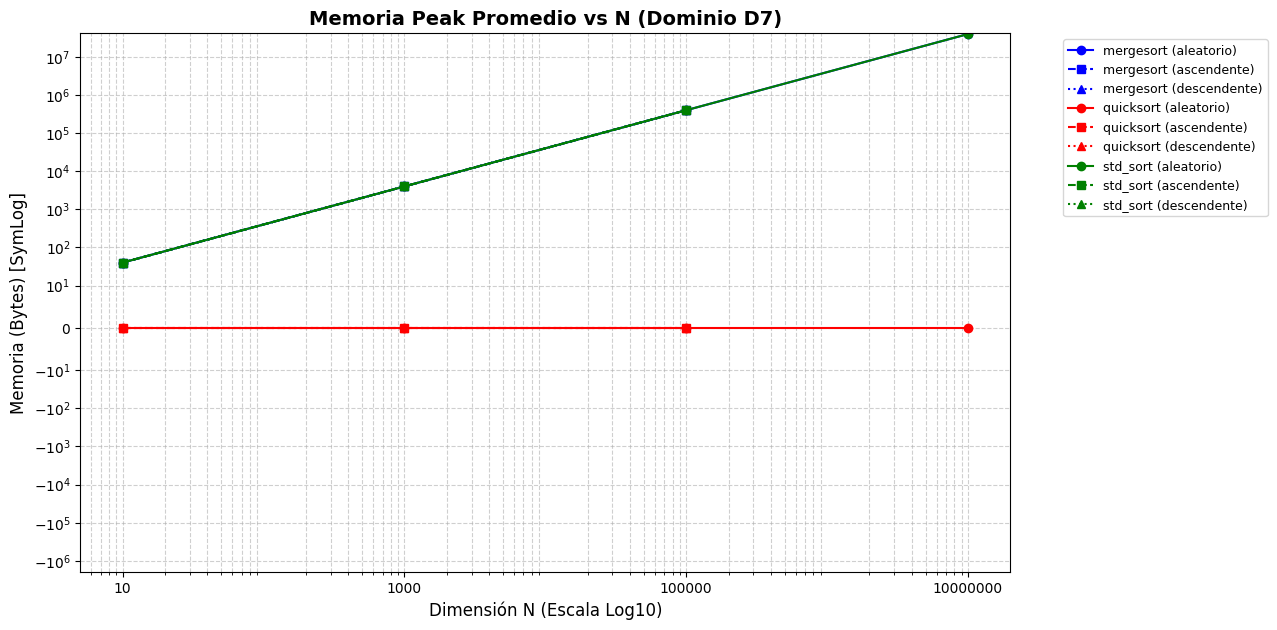
\includegraphics[width=0.75\textwidth]{../code/sorting/plots/memoria_vs_n_D7.png}
    \caption{Consumo peak de memoria en ordenamiento (Dominio D7). La superposición de las curvas inferiores valida el enfoque in-place.}
    \label{fig:sort_mem}
\end{figure}

\subsection{Multiplicación de Matrices}

Este experimento demuestra cómo las constantes de la notación Big-$\mathcal{O}$ afectan en la práctica. Primero, vemos que las curvas de matrices densas, diagonales y dispersas son iguales; esto confirma que los algoritmos procesan todo de la misma forma al no tener optimizaciones para saltarse los ceros.

En el \textbf{tiempo de ejecución} (Figura \ref{fig:mat_tiempo}), podemos ver aunque en teoría \texttt{Strassen} ($\mathcal{O}(n^{2.81})$) es más rápido que \texttt{Naive} ($\mathcal{O}(n^3)$), en la gráfica siempre se demora más. Por ejemplo, con $N=1024$, Naive termina en $\approx 1.6$ ms, mientras que Strassen se termina demorando más de $160.000$ ms. Esto ocurre porque el costo de la recursión en Strassen es mucho más pesado que correr los tres \texttt{for} simples de Naive para matrices de $N \le 1024$.
\begin{figure}[H]
    \centering
    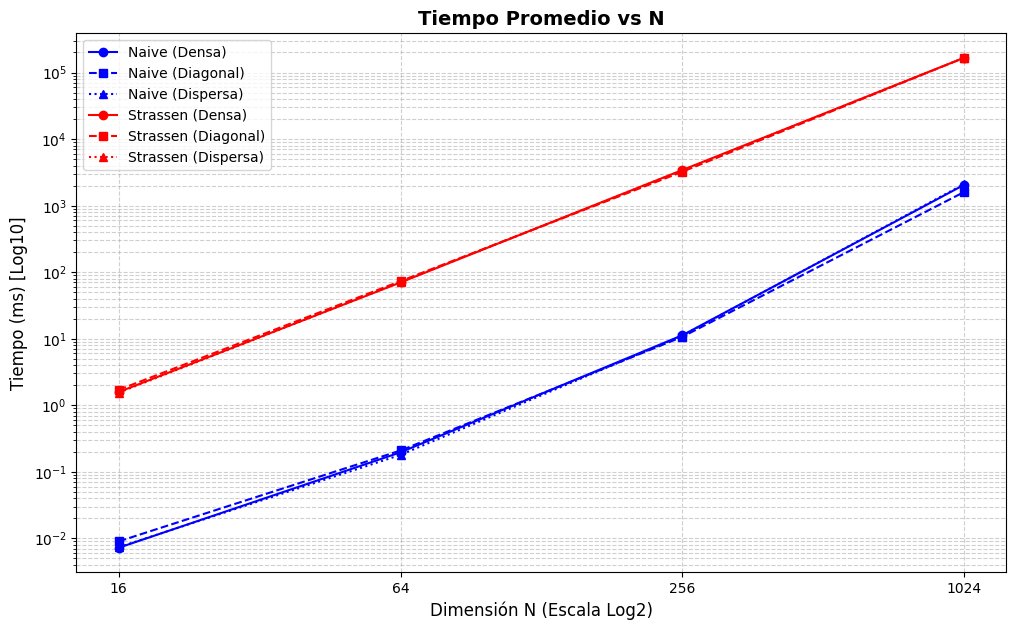
\includegraphics[width=0.75\textwidth]{../code/matrix_multiplication/plots/tiempo_vs_n_matrices.png}
    \caption{Tiempos promedio de ejecución en matrices. Escala Log-Log.}
    \label{fig:mat_tiempo}
\end{figure}

En cuanto a la \textbf{memoria consumida} (Figura \ref{fig:mat_mem}), al sobrecargar \texttt{new} registramos toda la memoria solicitada en el Heap durante la multiplicación. El método \texttt{Naive} (línea azul) solo gasta lo necesario para guardar la matriz con el resultado final. Por el contrario, \texttt{Strassen} (línea roja) consume muchísima más memoria porque la recursión lo obliga a estar creando varias submatrices temporales de $N/2$ en cada paso, lo que dispara su consumo.

\begin{figure}[H]
    \centering
    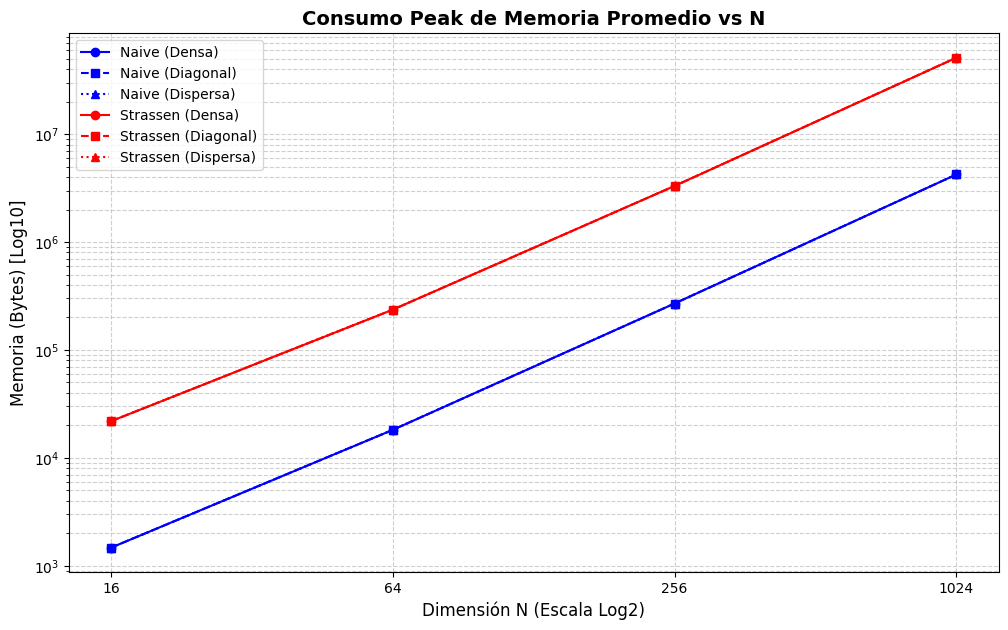
\includegraphics[width=0.75\textwidth]{../code/matrix_multiplication/plots/memoria_vs_n_matrices.png}
    \caption{Memoria auxiliar dinámica peak en matrices. Escala Log-Log.}
    \label{fig:mat_mem}
\end{figure}